%\section{Datenerfassung an der Charité}
information über copra (fridtjof ausquetschen). bla bla bla

Die Daten wurden vor dem Export pseudonymisiert, indem patientenbezogene Daten wie Name und Geburtsdatum entfernt wurden. Insbesondere werden Zeitpunkte nicht in absoluter Form angegebenen, sondern in Relation zum Beginn des Krankenhausaufenthalts des entsprechenden Patienten. Rückschlüsse auf die Identität der Patienten, deren Daten hier betrachtet werden, sind somit ausgeschlossen. Eine Zuordnung der erfassten Werte und Freitexte untereinander zum gleichen Patienten bleibt aber in Form einer eindeutigen Zahlenkombination weiterhin möglich.

Nach dem Export lagen die Daten in Form mehrerer Datendateien vor. \texttt{patienten.csv} enthält Metainformationen über die betrachteten Patienten. Separat gibt \texttt{delir.csv} für jeden Patienten an, ob für diesen während seines Aufenthalts ein Delir diagnostiziert wurde. Letztendlich geben die beiden Dateien \texttt{scores1.csv} und \texttt{scores2.xlsx} Aufschluss über die erfassten Scores und eingetragenen Freitexte. Jede Zeile enthält hierbei jeweils die VarID, den betreffenden Patienten, den Zeitpunkt sowie den eigentlichen erfassten Wert. Bei der VarID handelt es sich um einen ganzzahligen Wert, mit der jede Art von auf der Intensivstation erfasstem Wert bzw. eingetragenem Text intern repräsentiert und eindeutig identifiziert wird (siehe Tabelle \ref{table:varids}).

\section{Übersicht über die vorliegenden Daten} \label{section:vorliegende_daten}

Der mir für diese Arbeit zur Verfügung stehende Datensatz enthält Informationen über insgesamt 1357 Patienten-Aufenthalte auf den Intensivstationen der Charité Berlin, die allesamt im Zeitraum von XXX 2019 bis XXX 2020 stattfanden. Jeder Aufenthalt wird über eine numerische, inkrementell aufsteigende Nummer\footnote{in den exportierten Datensätzen als n\_ID bezeichnet} eindeutig identifiziert. Hierbei gilt es zu beachten, dass ein Patient bzw. eine Patientin, der/die im Laufe seiner/ihrer Behandlung mehrere Male auf eine Intensivstation verlegt wird, für jeden separaten Aufenthalt eine neue Identifikationsnummer erhält. Für jeden Patient/für jede Patientin liegen Informationen über das Geschlecht, BMI\footnote{Body-Mass-Index}, das Alter zum Zeitpunkt der Aufnahme und ob während des Aufenthalts ein Delir\footnote{F05.* gemäß ICD-10} diagnostiziert wurde, vor. Weiterhin ist die Dauer des Aufenthalts auf der Intensivstation vermerkt, sowie ob der Patient/die Patientin während seines/ihres Aufenthalts verstorben ist. Die Mortalität während des Aufenthalts lag bei etwa 17\% ($n=225$). Die beobachteten Aufenthalte verliefen über Zeiträume von wenigen Stunden bis zu mehreren Monaten. Die mittlere Aufenthaltsdauer während des Beobachtungszeitraums liegt bei etwa 7,2 Tagen, der Median beträgt 3,2 Tage. Fast die Hälfte aller Aufenthalte endete also nach weniger als drei Tagen. Nur etwas mehr als ein Viertel der Patienten ($n=375$) wurden für eine Woche oder länger auf der Intensivstation behandelt.

Für jeden Patienten werden während der Dauer seines Aufenthalts medizinische Scores (siehe Abschnitt \ref{section:scores}) bestimmt sowie Visitentexte geschrieben. Die Visitentexte werden digital erfasst und liegen im Unicode-Zeichensatz vor, folgen allerdings im Allgemeinen keinem einheitlichen Muster. Es handelt sich also um Freitexte, und es liegt im Ermessen der behandelnden Ärzte bzw. Pflegekräfte, einen aussagekräftigen Text zu formulieren. Ebenso können sich Faktoren wie Zeitdruck oder Stress auf Umfang und Genauigkeit der eingetragenen Texte auswirken(CITE).
%Bei den erfassten Scores handelt es sich um medizinische Bewertungssysteme, bei denen die Verfassung des betrachteten Patienten anhand klar definierter Regeln anhand einer Punktzahl bewertet wird(CITE). Häufig beziehen sich die Scores dabei nur auf einen kleinen Teil der Gesamtverfassung des Patienten, beispielsweise auf den Grad der Sedierung (RASS) oder auf das Schmerzempfinden, sofern dieses nicht vom Patienten selber mitgeteilt werden kann (BPS).
%Die in der vorliegenden Arbeit betrachteten Scores weisen es sich um Scores mit einem hohen Grad an Spezifität. Das Ziel solcher Scores ist es nicht, den Gesundheitszustand eines Patienten in seiner Gesamtheit zu erfassen, sondern eher einen klar abgrenzbaren Teilbereich davon \citep{marxIntensivmedizin2015c}. 
Tabelle \ref{table:varids} enthält eine Übersicht über alle Scores und Freitexte, die in dem gegebenen Datensatz erfasst wurden.

\begin{table}[htb] %here > top > bottom
    \centering
    \begin{tabular}{llr}\toprule
        \textbf{VarID}	&\textbf{Name} &\textbf{Wertebereich} \\\midrule
        20512769    & Glasgow Coma Scale (GCS)          & $v \in \interval{3}{15}$ \\
        20512801    & Behavior Pain Scale (BPS)         & $v \in \interval{3}{12}$ \\
        20512802    & Delirium Detection Score (DDS)    & $v \in \interval{3}{35}$ \\
        22085815    & Visite\_ZNS                        & Freitext \\
        22085820    & Visite\_Oberarzt                   & Freitext \\
        22085836    & Visite\_Pflege                     & Freitext \\
        22085897    & Ramsay Sedation Scale             & $v \in \interval{0}{6}$\footnote{Entgegen der ursprünglichen Spezifikation ist an der Charité zusätzlich eine Eintragung des Werts $0$ (für "wach, voll orientiert") möglich.} \\
        22085911    & NRS/VAS (Visual Analogue Scale)   & $v \in \interval{0}{10}$ \\
        22086067    & Vigilanz                          & Freitext* \\
        22086158    & Richmond Agitation Sedation Scale (RASS) & $v \in \interval{-5}{4}$ \\
        22086169    & CAM-ICU                           & $v \in \{	\text{neg.}, \text{pos.}, \text{unmögl.} \}$ \\
        22086170    & BPS-Bewertung                     & Freitext* \\
        22086172    & NRS/VAS Bedingungen               & Freitext* \\\bottomrule
    \end{tabular}

    \caption{Übersicht aller erfassten Scores und Freitexte}
    \label{table:varids}
\end{table}

Es folgt eine detailliertere Beschreibung derjenigen Werte, die für den Inhalt dieser Arbeit besonders hohe Relevanz haben:

\paragraph{Glasgow Coma Scale}
Bei der Glasgow Coma Scale (GCS) wird die Schwere einer möglicherweise vorliegenden Bewusstseinsstörung anhand von drei Kategorien (Augenöffnen, verbale Antwort und motorische Reaktion) ermittelt. In jeder Kategorie wird eine Punktzahl ermittelt, die dann zu einem Endergebnis aufsummiert werden. Insgesamt sind so Werte zwischen einschließlich 3 und 15 möglich \citep{teasdaleAssessmentComaImpaired1974,marxIntensivmedizin2015c}.

\paragraph{RASS}
Die Richmond Agitation Sedation Scale (RASS) ist eine zehnstufige Messzahl, die den Grad der Sedierung eines Intensivpatienten beschreibt. Mögliche Werte liegen zwischen $-5$ ("unarousable"/"nicht erweckbar") und $4$ ("combative"/"streitlustig"). Bei den betrachteten Patienten wurde der Wert $0$ ("aufmerksam und ruhig") am Häufigsten erfasst, was dem erwünschten Wert entspricht, solange keine Sedierung indiziert ist. Die Autoren der Skala empfehlen eine Reihe von Stimuli, die dem Patienten präsentiert werden sollen, um eine besonders genaue Bestimmung des richtigen Wertes zu ermöglichen \citep{sesslerRichmondAgitationSedation2002a}. Die RASS weist eine hohe Reliabilität und Validität auf und gilt im deutschsprachigen Raum als Goldstandard zum Monitoring der Sedierungstiefe \citep{marxIntensivmedizin2015c, muellerAnalgesieSedierungUnd2015}.

\paragraph{CAM-ICU}
bla bla bla %https://www.ai-online.info/images/ai-ausgabe/2009/10-2009/2009_10_592-600_Confusion%20Assessment%20Method%20for%20Intensive%20Care%20Unit%20zur%20routine-maessigen%20Kontrolle%20.pdf

\paragraph{NRS/VAS (Visual Analogue Scale)}
bla bla bla

\paragraph{Visite\_ZNS, Visite\_Oberarzt und Visite\_Pflege}
bla bla bla (Fridtjof fragen)

%hier histogramme mit den erfassten werten der einzelnen scores.

\subsection{Exemplarische Vorstellung eines Patienten} %z.b. 0430
Aufenthalt des Patienten hier detailliert beschreiben, und seinen Scatterplot einfügen (aber noch ohne Pfeile).

\subsection{Generierung von Schlüssel-Wert-Paaren}
Eine besondere Herausforderung stellte dar, dass die verschiedenen Werte und Texte zu unterschiedlichen Zeiten und unabhängig voneinadner eingetragen werden. Die Informationen über Zeitpunkt und Art der Eintragung sowie der eigentliche Wert liegen jeweils als Tripel in Form mehrerer Log-Dateien vor. Bei den Visitentexten entspricht der eingetragene Text dem Wert der Eintragung.

Um ein Machine-Learning Modell aus dem Bereich des supervised learnings zu trainieren ist eine hohe Anzahl von Trainingspaaren notwendig. Jedes Wertepaar enthält einen Text sowie einen medizinischen Score, der den in dem Text angegebenen Informationen über die Verfasssung des Patient/die Patientin möglichst genau entspricht. Zusammen bilden diese Paare die Grundlage der Modelle, selbstständig noch nicht gesehene Texte bewerten zu können.
Aufgrund der zeitlichen Unterschiede zwischen den Eintragungen von Texten und Scores erwies sich allerdings ebenjene Zuordnung zueinander als nicht trivial.

% Hier Bild mit 4 Patienten-Scatterplots! Bildbeschreibung: "Patient X ist der Patient, dessen Aufenthalt in Sektion 2.2.2 detailliert vorgestellt wurde."
\begin{figure}
    \centering
    \subfloat{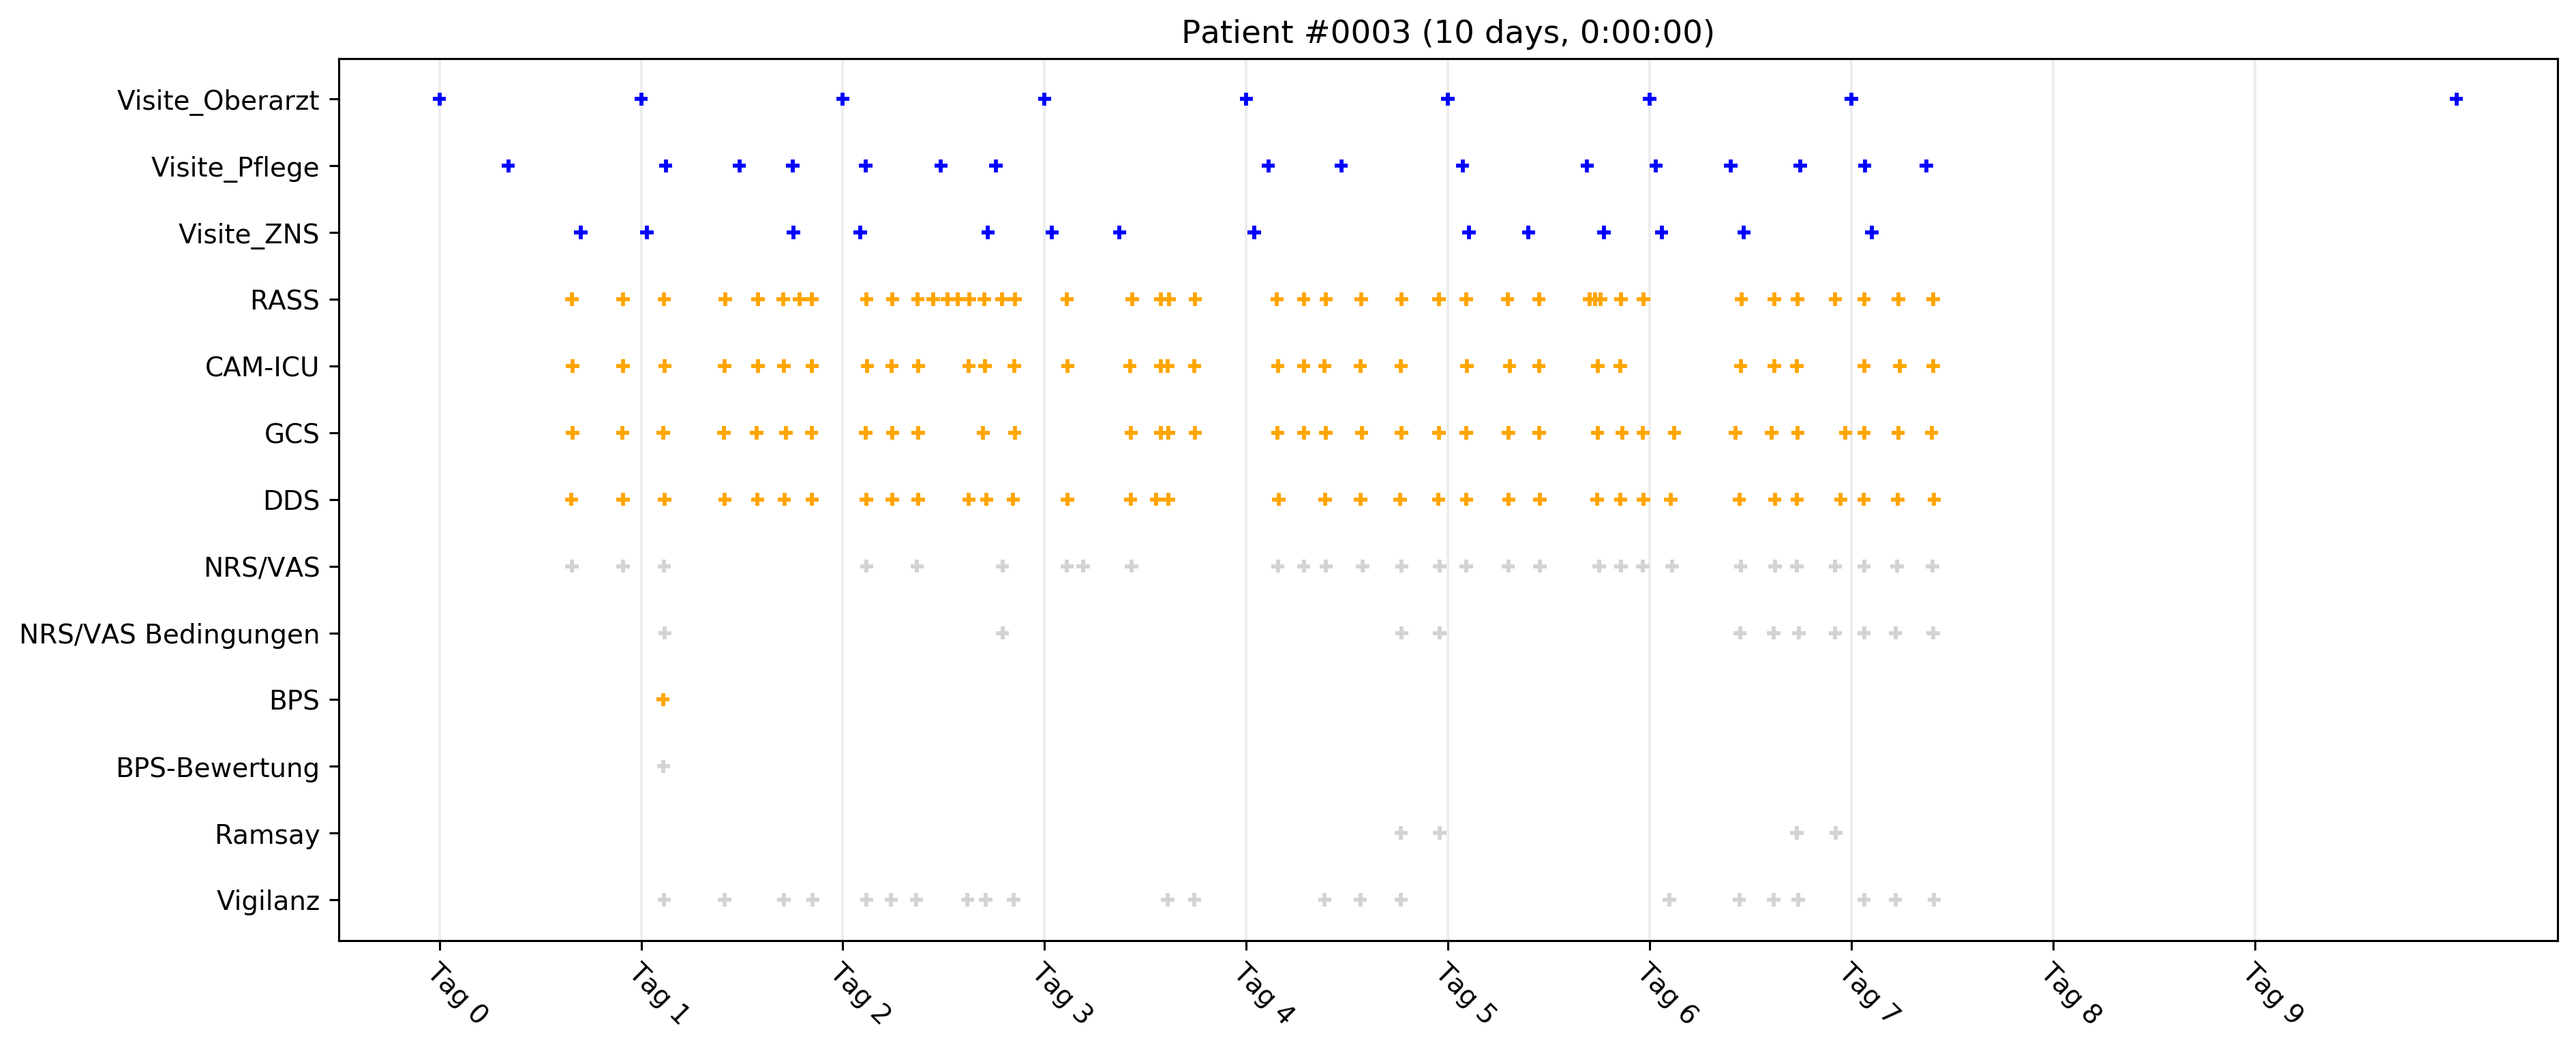
\includegraphics[height=2in]{patienten_scatters/patient_0003}} \\
    \subfloat{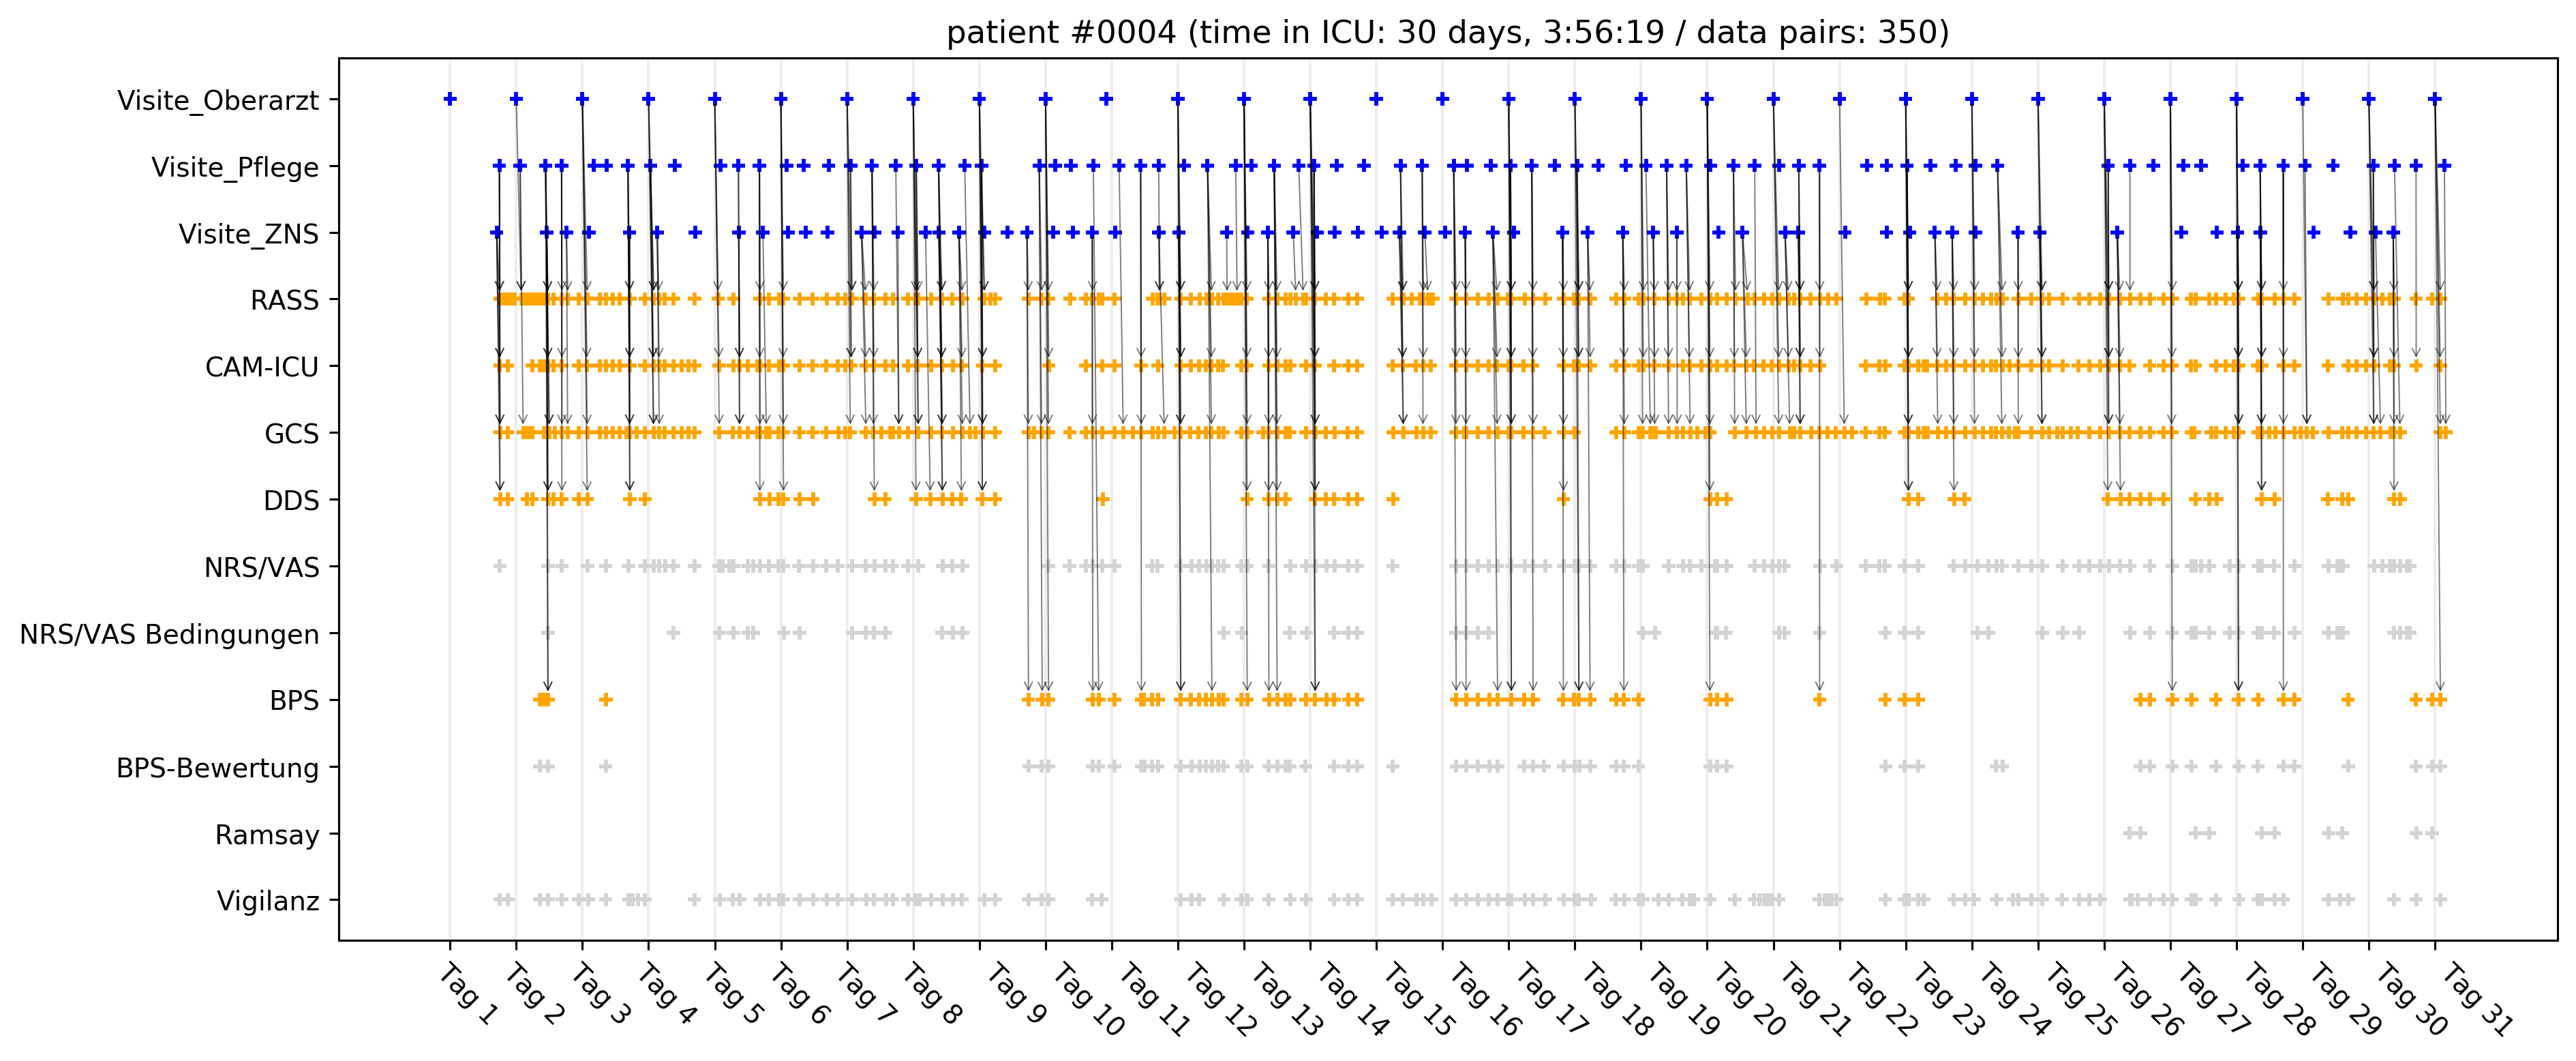
\includegraphics[height=2in]{patienten_scatters/patient_0004}} \\
    \subfloat{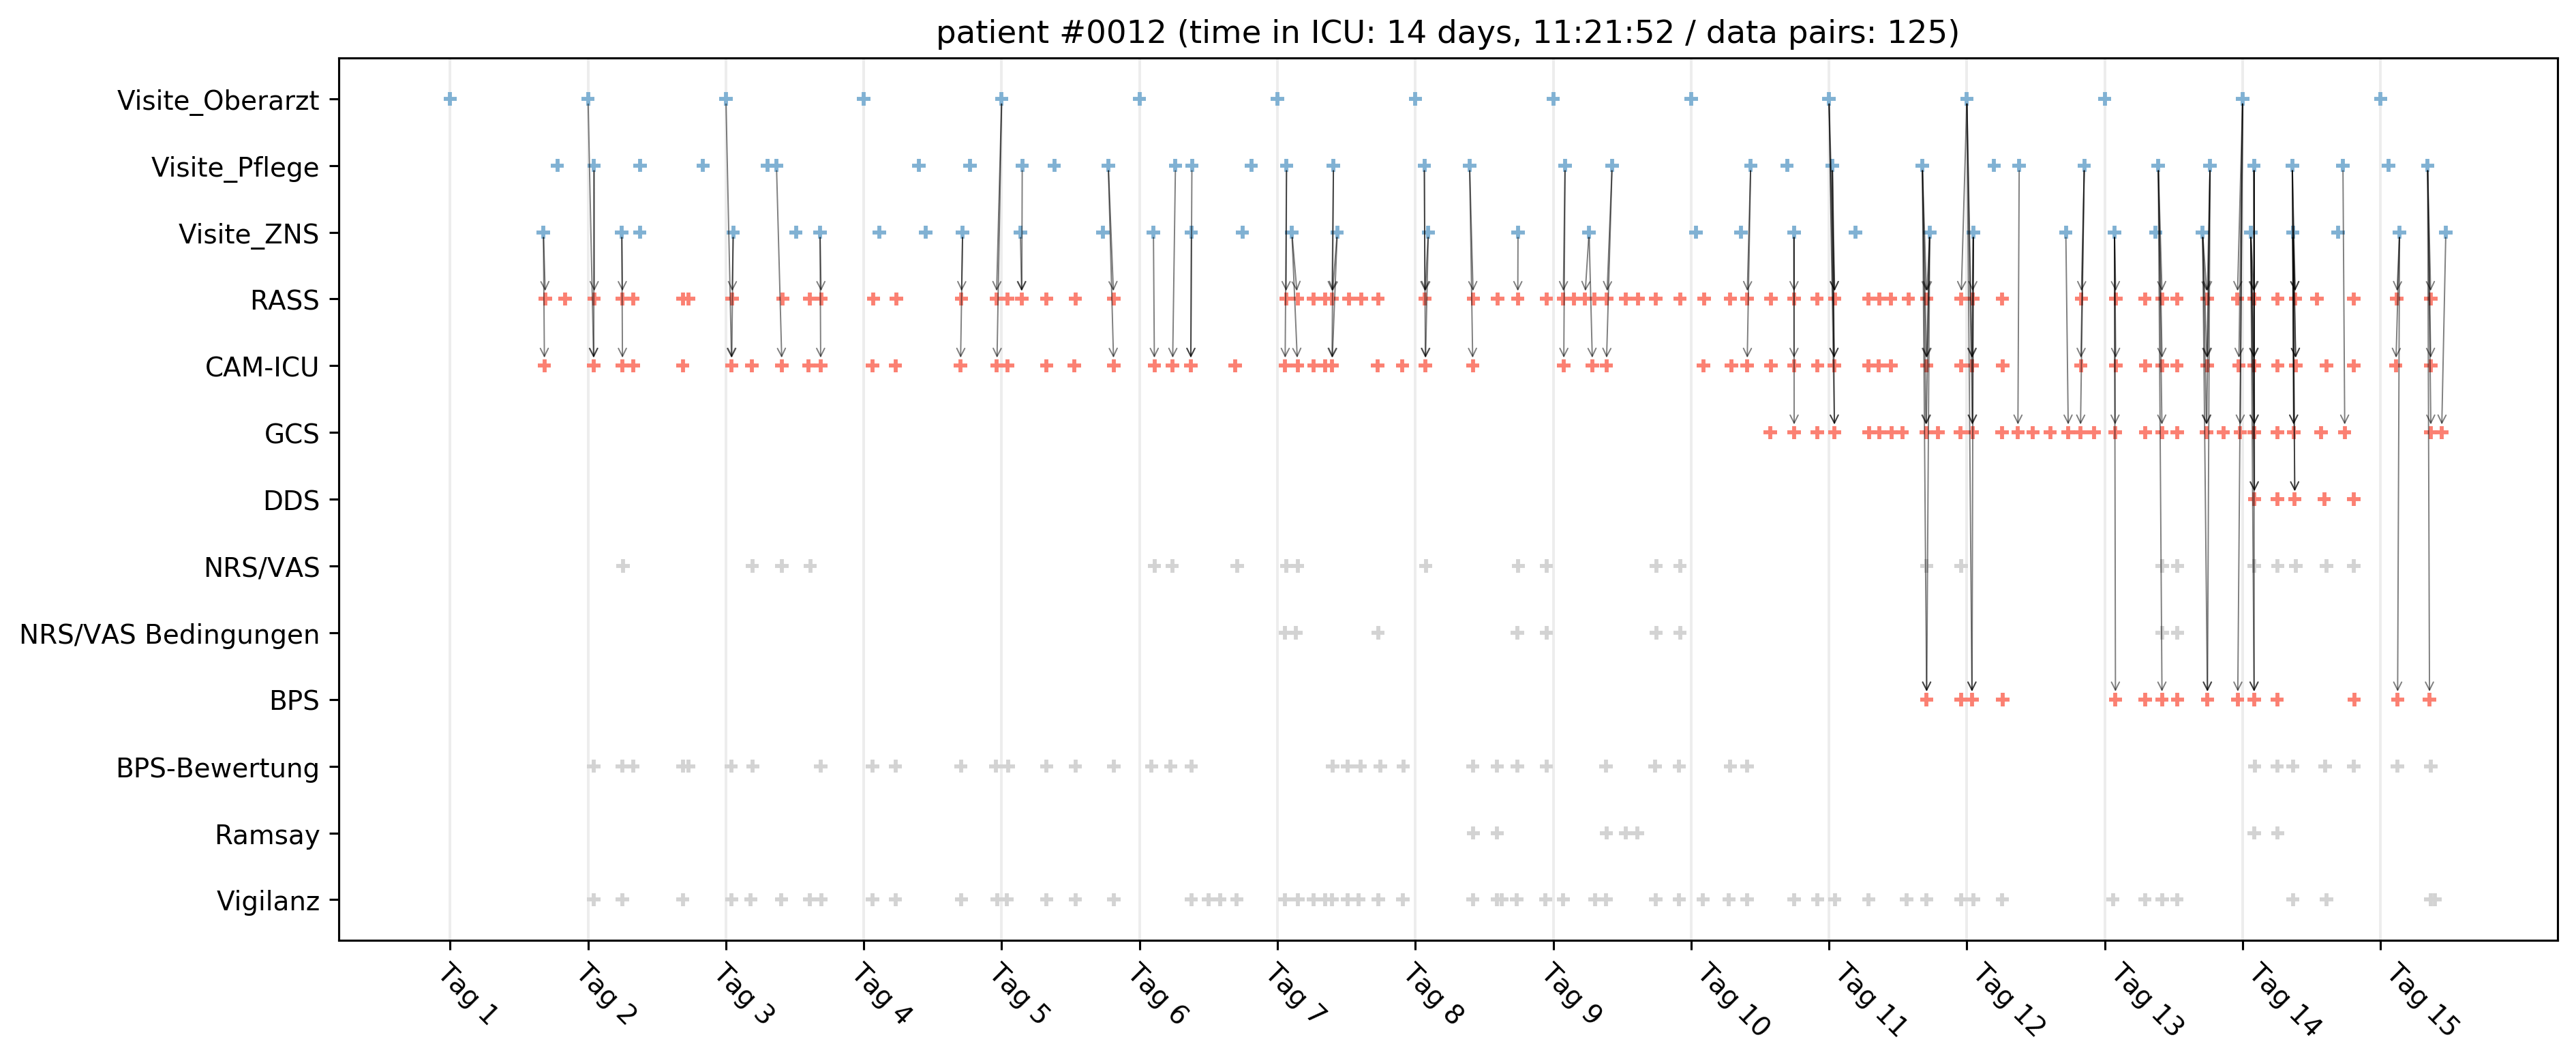
\includegraphics[height=2in]{patienten_scatters/patient_0012}} \\
    \subfloat{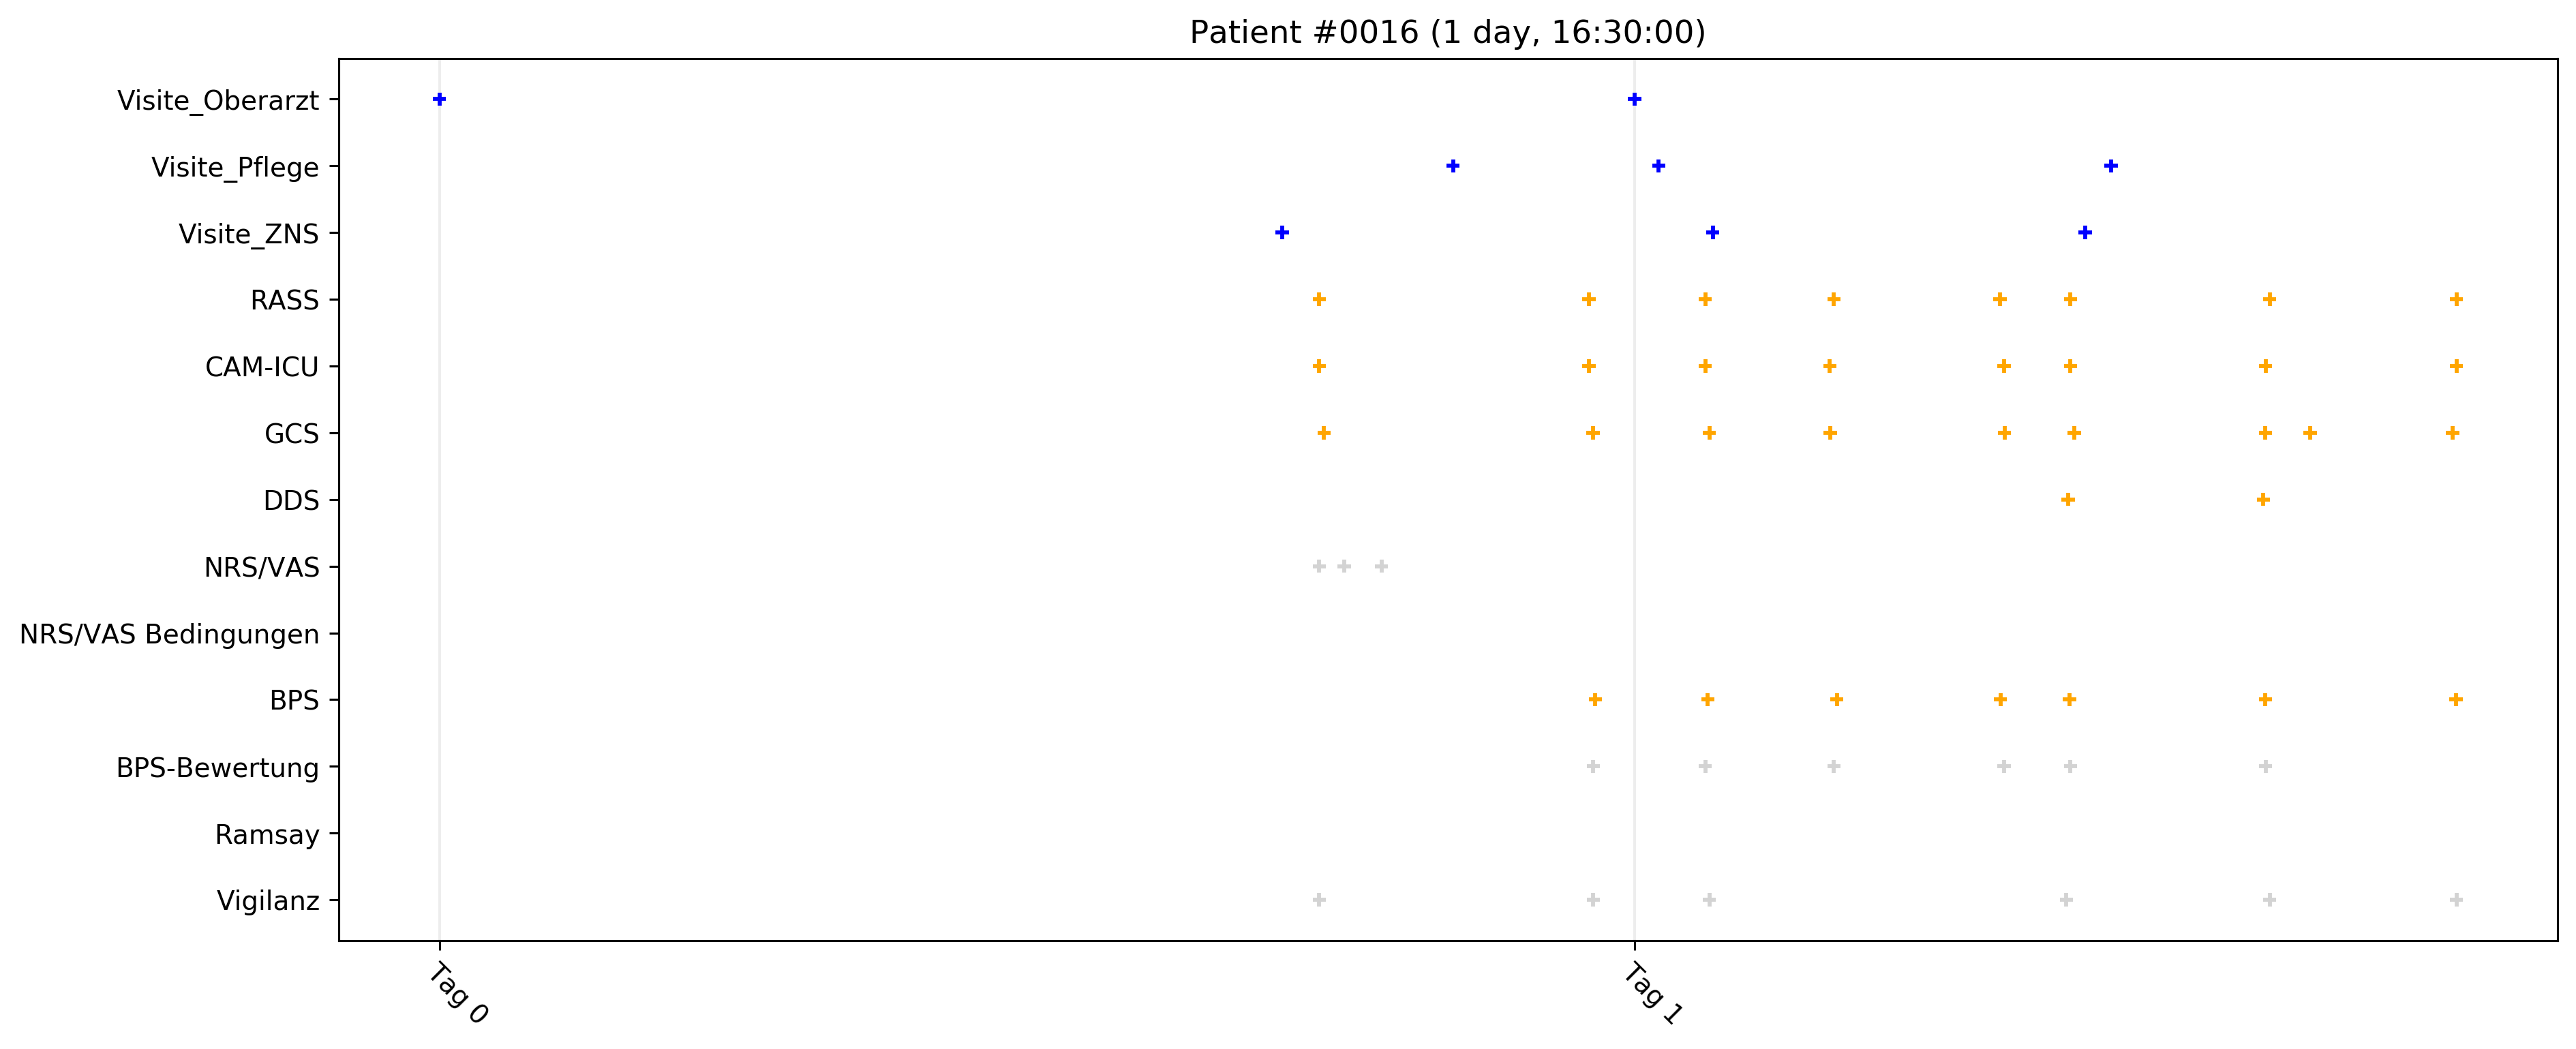
\includegraphics[height=2in]{patienten_scatters/patient_0016}} 
    \caption{Übersicht der erfassten Werte einiger Patienten}
    \label{fig:pat_example_scatterplots}
\end{figure}

\section{Genauigkeit der erfassten Daten}
Hier beschreiben, dass viele Texte nicht wirklich den Werten entsprechen. Das mache es schwerer, Modelle zu trainieren, und muss berücksichtigt werden. Gründe:
\begin{enumerate}
    \item Zeitdruck, Stress bei Ärzten, kann vorkommen dass sie einfach Wert vom letzten mal kopieren
    \item Werte können sich innerhalb von Minuten ändern (z.B. RASS von 0 auf -5)
    \item Weitere Gründe?
\end{enumerate}
Diese Grüunde sind aber nicht weiter Beobachtungsgegenstand der vorleigenden Arbeit. Dennoch muss das bei der Konzeption, Entwicklung und Bewertung beachtet werden, weil sie ohne weitere Maßnahmen möglicherweise eine obere Schranke für die Performance der Modelle darstellen.

%   * **Vergleich der verschiedenen Methoden, Wertepaare aus den Daten zu generieren**
%     * nearest value pairs
%     * last text observation carried forward
%     * Vergleich anhand der scatter plots f. **einen** geeigneten Patienten
%   * Abb: Liniendiagramm Anzahl key-werte paare pro predicted varid sowie max cutoff time